\section{Introduction to Data Analysis: Data Classification}
\label{sec:data_analysis}

\subsection{Supervised Classification}
\textcolor{blue}{\textbf{Question 1:}}
\textit{Enumerate main supervized classification techniques and describe them in few lines.}

%~~~~~~~~~~~~~~ANSWER~~~~~~~~~~~~~~
Supervised Classification is one of the two broad types of digital classification methods used by the majority of image processing systems to analyse remote sensing images. It requires selection of an appropriate classification scheme, and then identification of training areas in the image that best represents each class. In supervised classification, the analyst identifies in the image homogenous representative areas of different land use and land cover types (information classes) of interest. These are called \textit{training areas} or \textit{training samples}. 

The three distinct stages of Supervised Classification are training, classification and output. Training is the identification of a sample of pixels of known classes gathered from reference data, such as field visits, existing maps, reports and aerial photographs. These could be e.g. water, sand, dirt, roads, clouds etc. The key characteristics of selecting training areas are shape, location, number and uniformity.



Some typical Supervised Classification techniques are listed and described below:
\begin{enumerate}
    \item \textbf{k-Nearest Neighbours (k-NN):} The most simple classification algorithm where the principle is to find the \textit{k} closest data in the dataset to determine its class. 
    First a distance has to be defined, which is not always easy.

    
    \item \textbf{Maximum Likelihood:} A simple classifier based on the probability distribution.
    It assumes the data follows a known probability distribution (typically normal or Gaussian distr.) for each class.
    ML estimates the probability that a given data point belongs to each possible class and assigns it to the class with the highest likelihood.

    \begin{equation*}
        C^* = \underset{C_i}{\operatorname{argmax}} \, P(C_i \mid o)
    \end{equation*}

    
    \item \textbf{Bayesian Classification:}
    Based on the bayesian rule where given an observation \textit{o}, the \textit{prior} (a priori probability), is described as:
    \begin{equation*}
        P(C_i \mid o) = \frac{P(o \mid C_i) P(C_i)}{P(o)}
    \end{equation*}
    where $P(C_i \mid o)$ is called \textit{posterior} (a posterior probability).

    More text??

    
    \item \textbf{Linear Classification:}
    The most simple classification rule, where the objective is to establish a hyperplane, \textit{HP}, that separates the data into two groups:
    \begin{equation*}
    \begin{split}
        &\mathcal{H} : w_0 + \vec{w} \cdot \vec{x} = 0 \\
        &\text{In a \textit{n}-D space:} \\
        &\mathcal{H} : w_0 + w_1 x_1 + w_2 x_2 + \cdots + w_n x_n = 0
    \end{split}
    \end{equation*}

    Linear Classification is only possible if the data is \textit{linearly separable}. If not, there are infinite solutions
    An example of Linear Classification is the Perceptron Algorithm, which bla bla
    
    
    \item \textbf{Neural Networks:}
    \item \textbf{Decision Trees:}
    \item \textbf{Concept Lattices:}
    \item \textbf{Support Vector Machine}
    \item \textbf{Random Forests:}
    \item \textbf{etc.}
\end{enumerate}



\textcolor{blue}{\textbf{Question 2:}}
\textit{Apply and compare the following algorithms:
\begin{enumerate}
    \item 1-NN (your programme)
    \item Neural Network    
\end{enumerate}
on 'Spain Beach' image or another of your choice}

\begin{enumerate}
    \item 1-NN 

    The first step is to select the data for our classes, which we select at random in predefined areas for 'land', 'beach', 'foam' and 'ocean' classes.
    \begin{figure}[!ht]
        \centering
        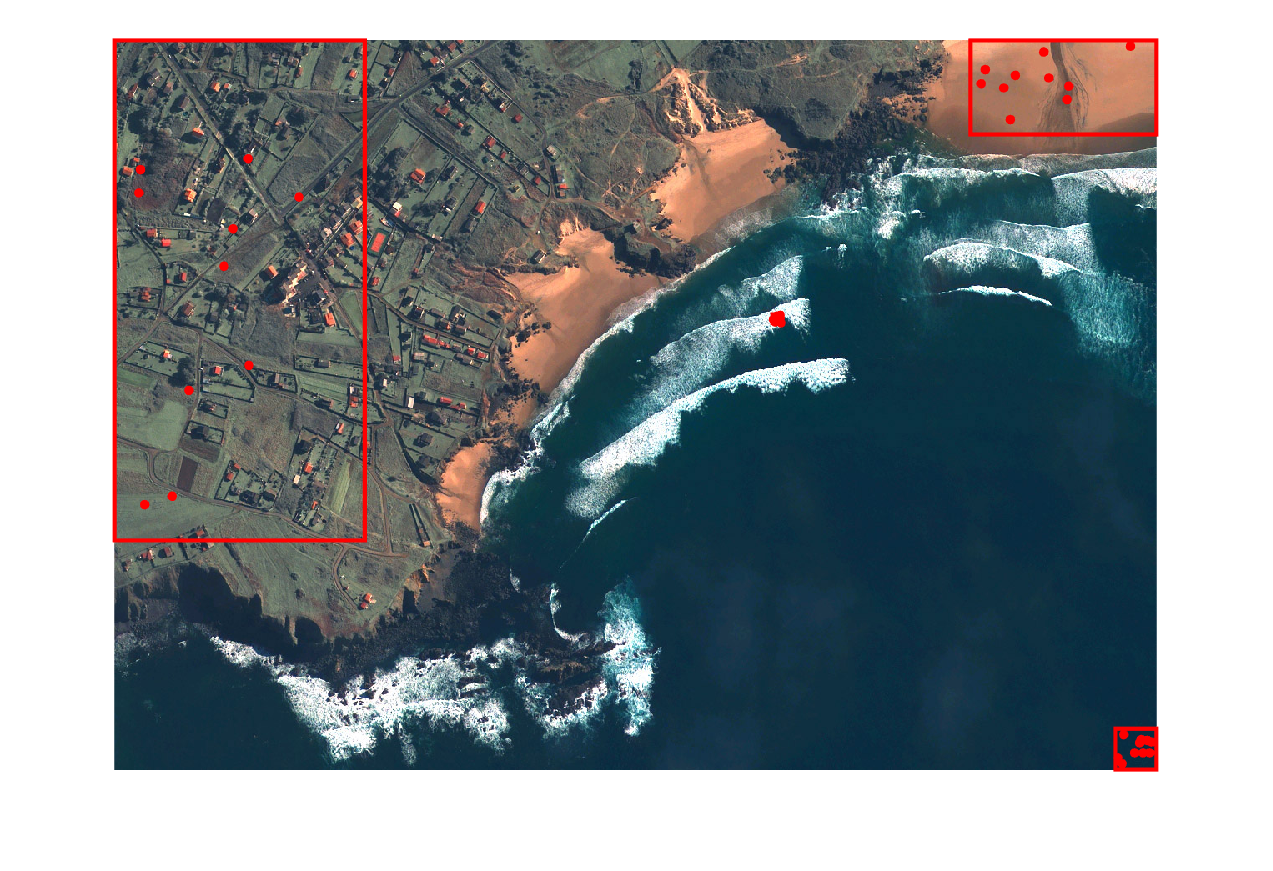
\includegraphics[width=0.45\linewidth]{Doc/Graphics/Part4/kNN_training_sets.png}
        \caption{Randomly selected training data}
    \end{figure}

    The output of the algorithm gives us the beach we want to extract
    \begin{figure}[!ht]
        \centering
        \begin{subfigure}{0.45\textwidth}
            \centering
            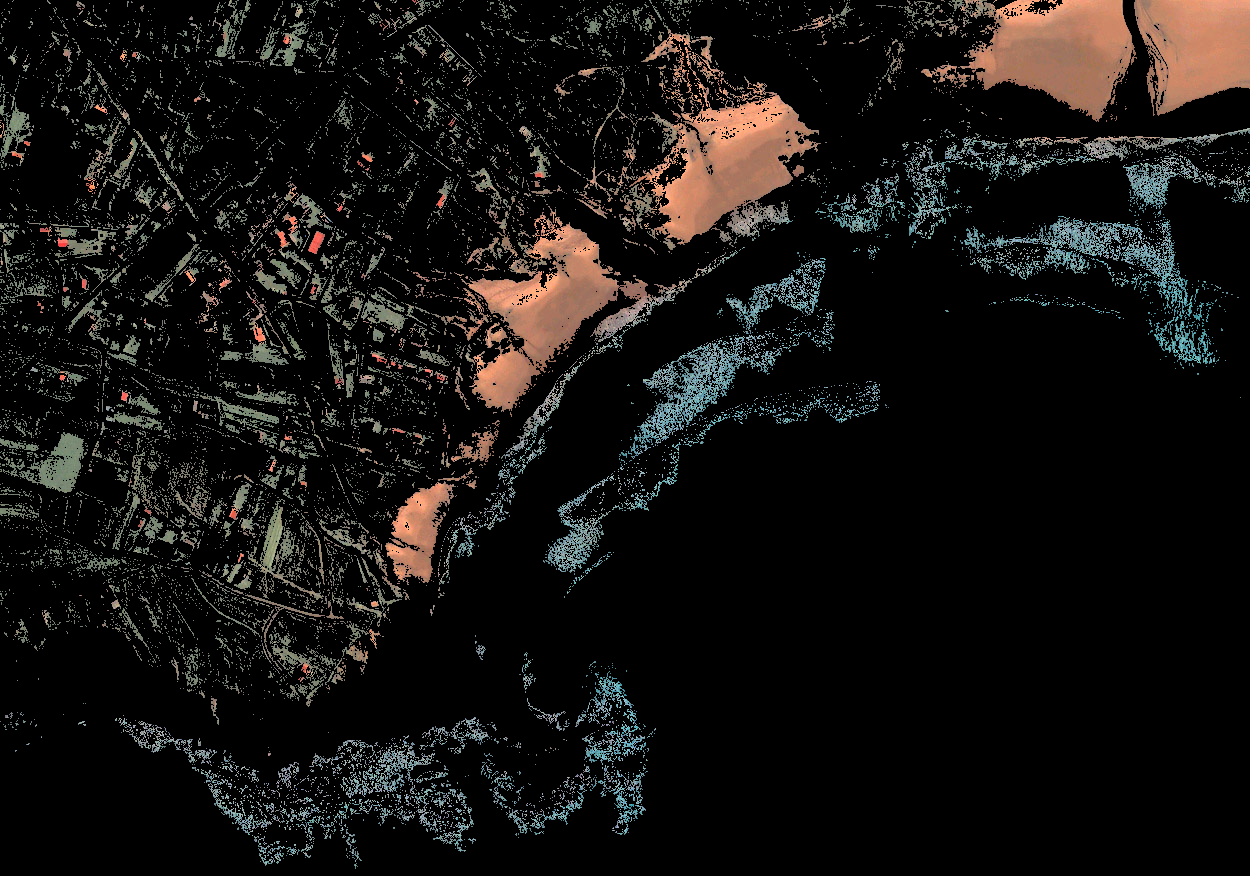
\includegraphics[width=\textwidth]{Doc/Graphics/Part4/kNN_classified_beach.png}
            \caption{Raw output}
        \end{subfigure} \hfill
        \begin{subfigure}{0.45\textwidth}
            \centering
            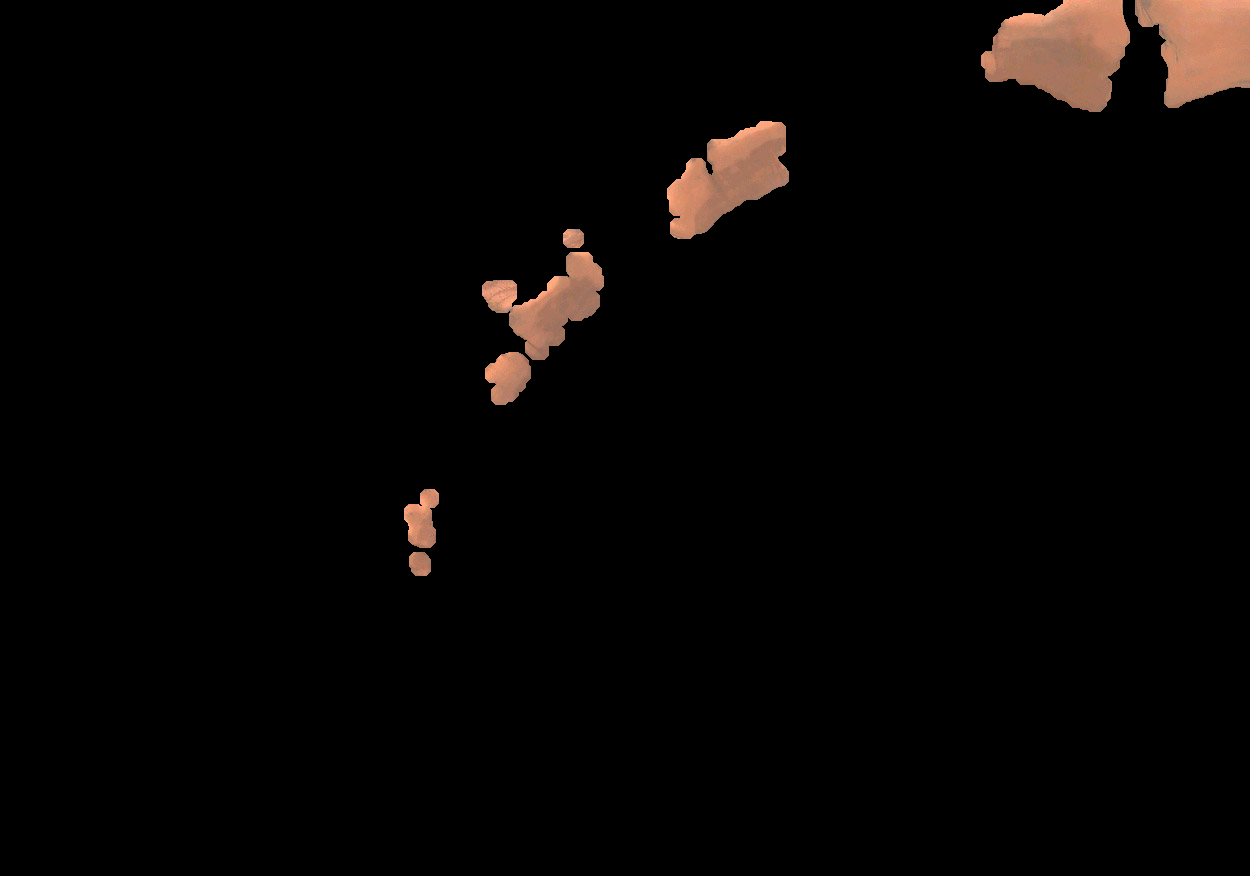
\includegraphics[width=\textwidth]{Doc/Graphics/Part4/kNN_masked_beach.png}
            \caption{Smoothened output}
        \end{subfigure}
        \caption{Extracted beach}
        \label{fig:enter-label}
    \end{figure}  
    \FloatBarrier
    
    \item Neural Network
    
    We select two sets of training data, which gives us two classes: 'beach' and 'not beach'. 
    \begin{figure}[!ht]
        \centering
        \begin{subfigure}{0.2\textwidth}
            \centering
            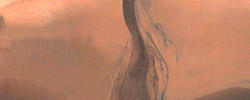
\includegraphics[width=\textwidth, angle=90]{Doc/Graphics/Part4/training_set_beach.png}
            \caption{Beach}
        \end{subfigure}
        \begin{subfigure}{0.4\textwidth}
            \centering
            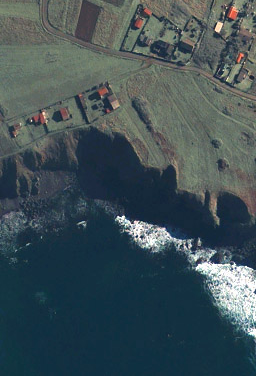
\includegraphics[width=0.5\textwidth, angle=90]{Doc/Graphics/Part4/training_set_other.png}
            \caption{Not beach}
        \end{subfigure}
        \caption{Training sets}
    \end{figure}
    \FloatBarrier

    The target assigned to beach RGB values is 1 and 0 for the rest. Training the network goes smoothly, and its output results in the following extraction of the beach:
    \begin{figure}[!ht]
        \centering
        \begin{subfigure}{0.45\textwidth}
            \centering
            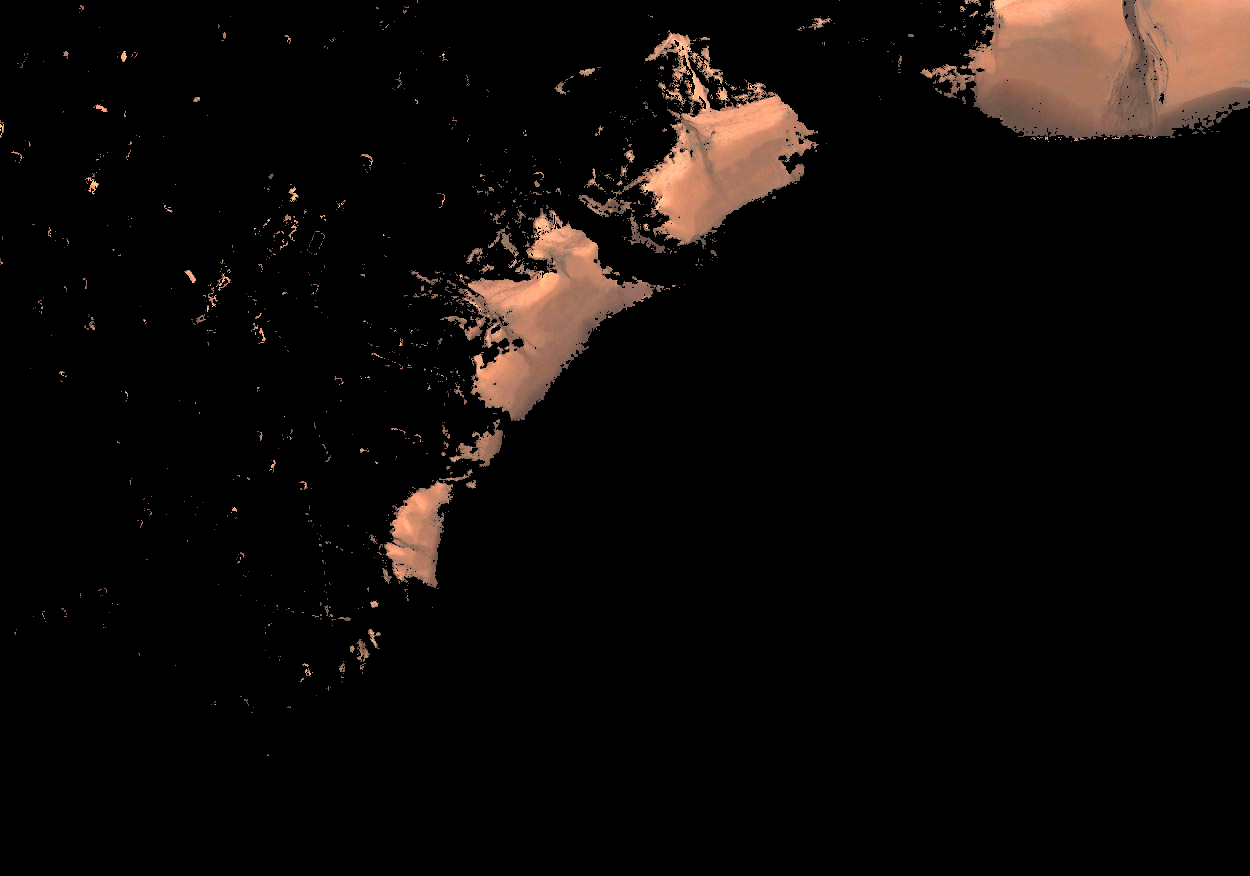
\includegraphics[width=\textwidth]{Doc/Graphics/Part4/nn_classified_beach.png}
            \caption{Raw output}
        \end{subfigure} \hfill
        \begin{subfigure}{0.45\textwidth}
            \centering
            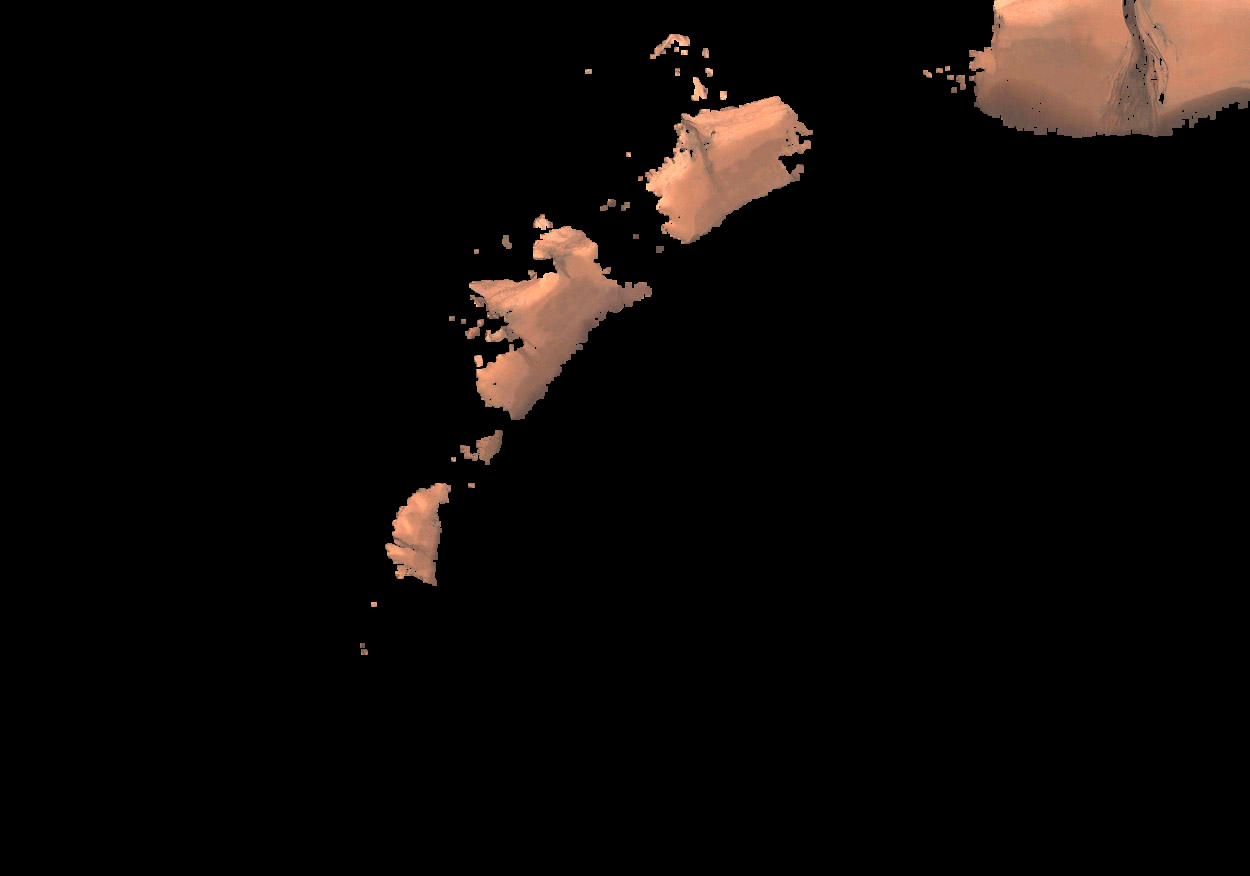
\includegraphics[width=\textwidth]{Doc/Graphics/Part4/nn_masked_beach.png}
            \caption{Smoothened output}
        \end{subfigure}
        \caption{Extracted beach}
        \label{fig:enter-label}
    \end{figure}
    \FloatBarrier

    \item Comparison

    There are two noticeable differences: speed and noise level. The neural network is much more performant in terms of speed and produces an output with much less noise and better classification (like the river delta in the top right corner).
\end{enumerate}



\textcolor{blue}{\textbf{Question 3:}}
\textit{Search on internet one of the two the following algorithms and apply it to the same image
\begin{enumerate}
    \item SVM
    \item Ramdom Forest
\end{enumerate}
}



% ~~~~~~~~~~~~~~ UNSUPERVISED CLASSIFICATION ~~~~~~~~~~~~~~~~~~
\newpage
\subsection{Unsupervised Classification}
\textcolor{blue}{\textbf{Question 4:}}
\textit{Enumerate main unsupervized classification techniques and describe them in few lines.}

Unsupervised Classification in essence reverses the process of supervised classification. It requires less input from the analyst to process the image, as the analyst does not predefined the land use and land cover types. However, the analyst can define the number of output classes required and spectral variance (such as the standard deviation, $\sigma$) within each class. The image is divided into those defined number of classes based entirely on the spectral data and with no prior knowledge of what land use and land cover types may be present in the image. 

\begin{itemize}
    \item \textbf{Clustering} 
    \subitem \textit{K-Means Algorithm}
    \subitem \textit{Kohonen Maps}
    \item \textbf{Regression}
    \item \textbf{Dimension Reduction}
    \subitem \textit{Principal Component Analysis} is the most efficient method for Dimension Reduction. It is based on the variance / covariance matrix, where the main eigenvalues are the most important. Associated eigenvectors describe the reduced state space.
\end{itemize}


\textcolor{blue}{\textbf{Question 5:}}
\textit{Apply the following algorithms with the dedicated objective
\begin{enumerate}
    \item k-means algorithm to define the four classes automatically and speed-up the classification process
    \item Pseudo-Inverse technique to estimate the position of a planet
    \item PCA technique to reduce the size of an image
\end{enumerate}
}

Principal Component Analysis (PCA)
\begin{figure}[!ht]
    \centering
    \begin{subfigure}{0.45\textwidth}
    \centering
        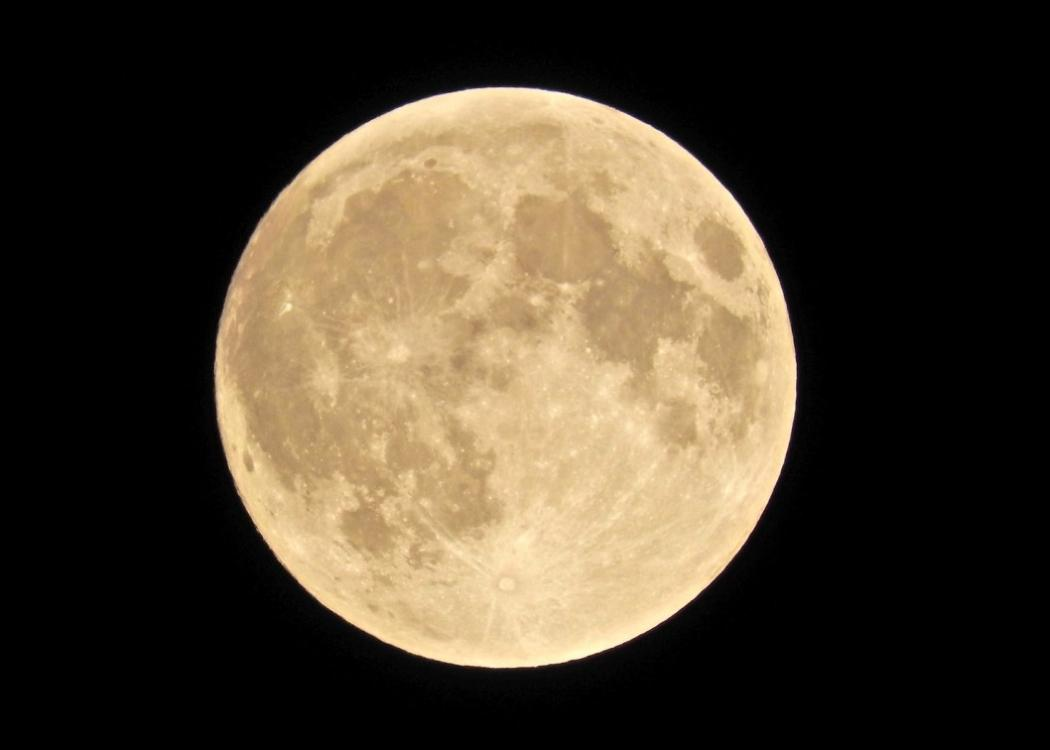
\includegraphics[width=\linewidth]{Doc/Graphics/Part4/PCA_im_original.png}
        \caption{Original}
    \end{subfigure}
    \begin{subfigure}{0.45\textwidth}
    \centering
        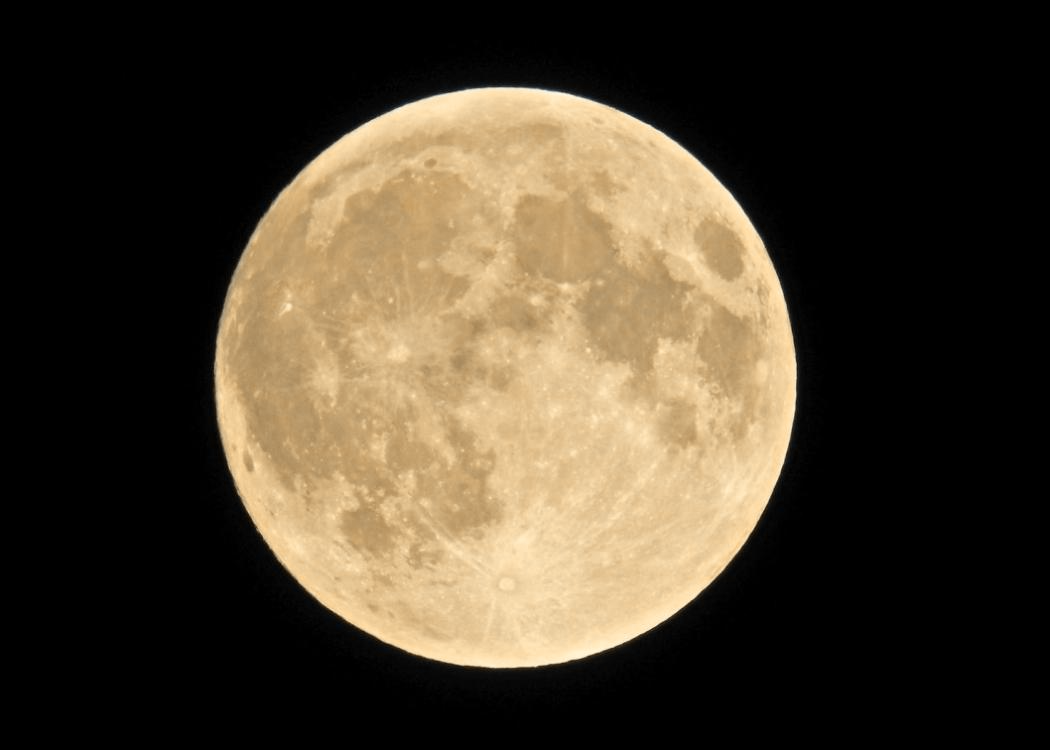
\includegraphics[width=\linewidth]{Doc/Graphics/Part4/PCA_im_reconstructed.png}
        \caption{Reconstructed}
    \end{subfigure}
    \caption{PCA compression}
    \label{fig:enter-label}
\end{figure}

\begin{figure}[!ht]
    \centering
    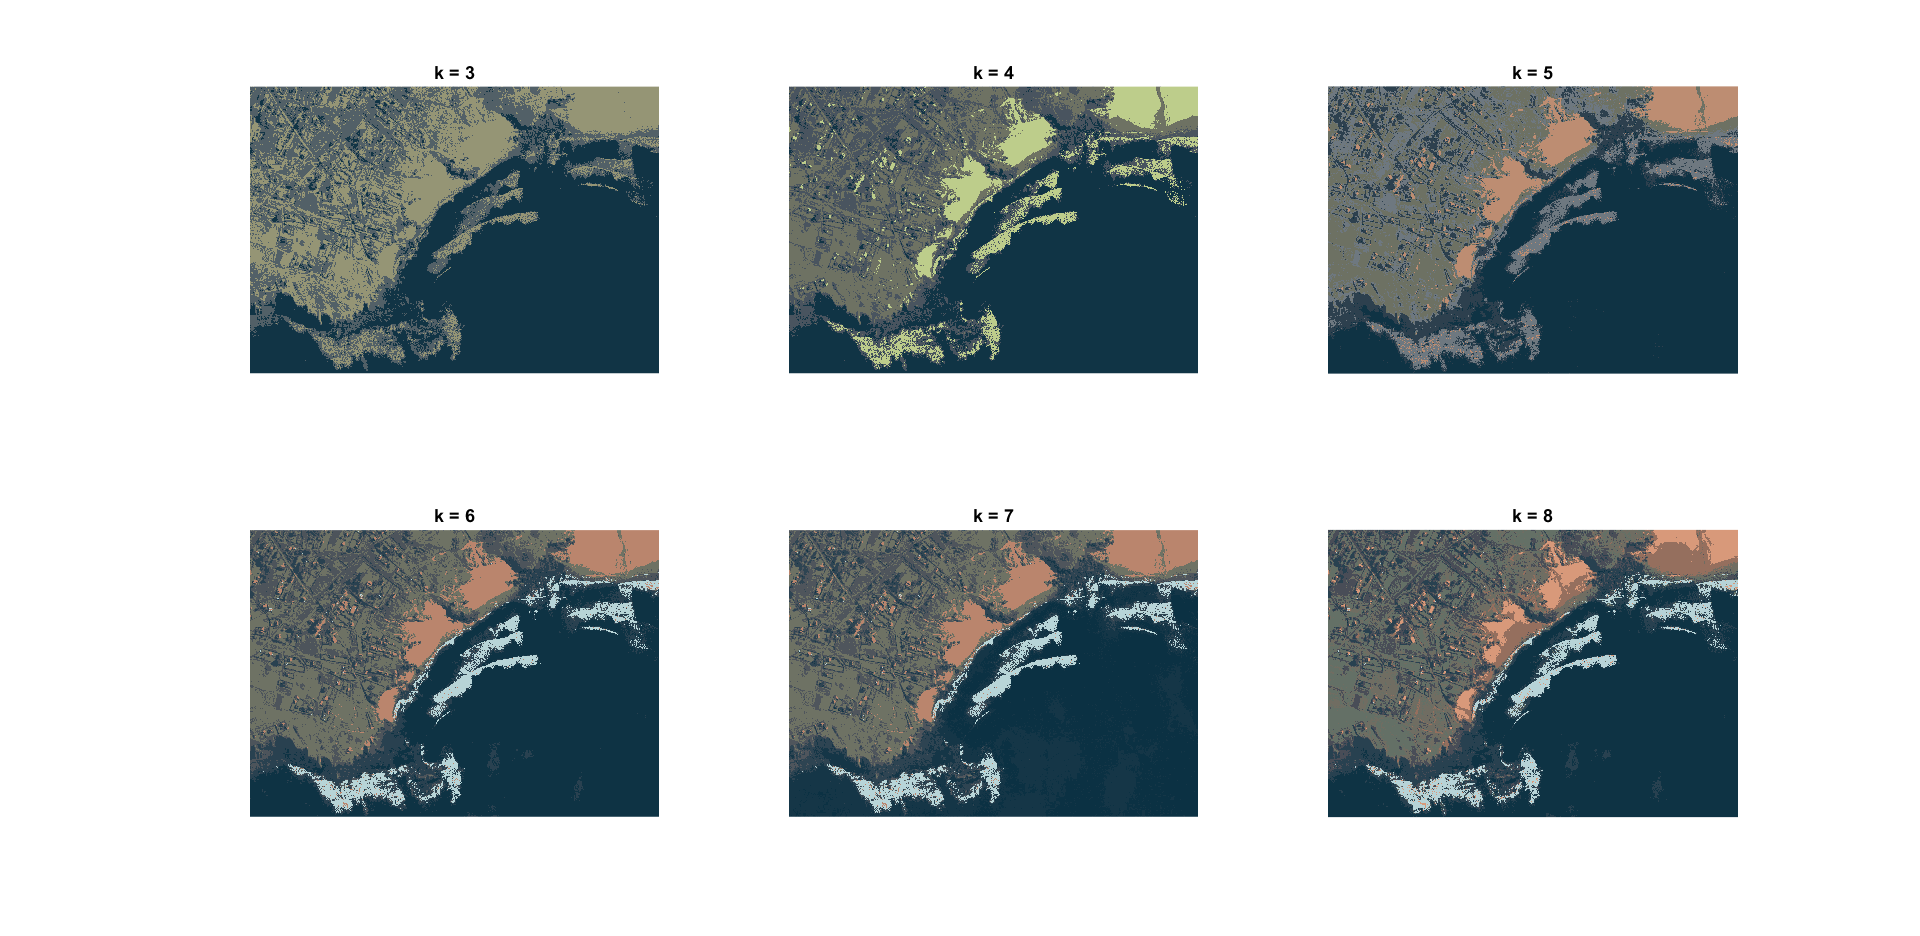
\includegraphics[width=\linewidth]{Doc/Graphics/Part4/kMeans_comparison.png}
    \caption{k-means clustering tests}
    \label{fig:enter-label}
\end{figure}